\documentclass[12pt]{article}

\usepackage{siunitx} % Provides the \SI{}{} and \si{} command for typesetting SI units
\usepackage{graphicx} % Required for the inclusion of images
\usepackage{amsmath} % Required for some math elements 
\usepackage{float}
\usepackage{amssymb}
%pakiety wspomagaj?ce i poprawiaj?ce sk?adanie tabel
\usepackage{supertabular}
\usepackage{array}
\usepackage{tabularx}
\usepackage{hhline}
\usepackage{graphicx} 
\usepackage{wrapfig}


\setlength\parindent{0pt} % Removes all indentation from paragraphs

\title{Newton's method} % Title

\author{Dominik \textsc{Koszkul} \\ Micha\l\ \textsc{Oleszczyk}} % Author name

\usepackage{geometry}

\newgeometry{tmargin=2cm, bmargin=2cm, lmargin=2cm, rmargin=2cm}

\begin{document}

\maketitle % Insert the title, author and date

\section{Introduce}

\subsection{Formulating optimization problem}
Problem, which needs to be solved, is to find minimum point in set of non-linear, multidimensional function. If function has more than one minimum, algorithm is looking for the nearest local minimum from the initial point. In this project, method to find these special points is \textit{Newton's method}. This algorithm allows to find local minimum points, but this particular method can be optimized by using other algorithm to find optimal step, which is used in the main optimization program. Thanks to this, whole algorithm can find the solution in a faster way. The objective function is presented in the following way
\begin{equation}
\min\limits_{x \epsilon \mathbb{R}^n} f(x) ,
\end{equation}
where $n \leqslant 5$. Newton's method is a gradient method without constraints. This means that minimum point is searched in $\mathbb{R}^n$.


\subsection{Newton's method}
Newton's method is a local optimization type algorithm. The algorithm is presented in the following steps:
\begin{enumerate}
\item compute $f(x^i)$ and gradient $\triangledown f(x^i)$,
\item compute direction $d^i=-H^{-1} \triangledown f(x^i)$,
\item compute step length in selected direction (use method which counts minimum in selected direction),
\item check stop criteria (if any criteria are fulfilled then stop and show results),
\item reply all from step 1 with new counted point $x^{i+1}$.
\end{enumerate}

 To implement the method, stop criteria should be also known. In this case we have three main stop criteria for Newton's method and one additional that ensures that program stops computing after exceeding maximum iterations number.

\subsubsection{Stop criteria}
\begin{enumerate}%[label=\arabic*.]
\item $ <grad f(x^i) \cdot grad f(x^i)> \leqslant \varepsilon_1 $ \\
Scalar product of the squared gradient of the function in point $x^i$ should be less or equal to $\varepsilon_1 $,
\item $ ||x^i-x^{i-1}|| \leqslant \varepsilon_2 $ \\
Euclidean norm of the distance between $x^i$ and $x^{i-1}$ points should be less or equal to $\varepsilon_2 $,
\item $ |f(x^i)-f(x^{i-1})| \leqslant \varepsilon_3 $ \\
Difference between values of the function in $x^i$ and $x^{i-1}$ should be less or equal to $\varepsilon_3 $,
\item maximum number of iterations.
\end{enumerate}  
If one from these four criteria is satisfied program stops computing and presents results. 

\subsubsection{Convergence}
Newton's method has a quadratic convergence - convergence rank equals two. This means that, if assumptions are fulfilled, the error decreases in a quadratic way along with the iteration number. In fact the convergence not always is. When the starting point is too far from minimum point the method may be divergent.

\subsubsection{Method constraints} \label{MC}
\textbf{Minimum in selected direction method} \\
Pure Newton's method after computing the direction has set step length which is equal to $1.0$. When the starting point is far from the local minimum the method will have huge amount of iterations and this is main reason of long computing time. In our implementation we used method, which can find the best step length in current iteration. This algorithm is \textit{bisection method with Goldstein test}. We chose this algorithm because in our program we have to compute the gradient and this method also uses the gradient to compute step length. Moreover this is one of the best method for Newton's algorithm. We can also set precision and thank to this manipulate speed of whole program.
\begin{figure}[H]
\begin{center}
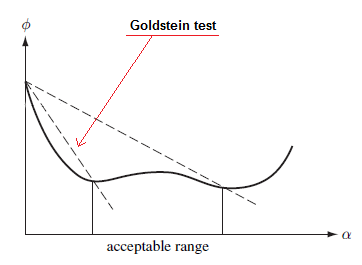
\includegraphics[scale=0.9]{images/goldstein.png}
\caption{Goldstein test example \cite{mathematics}}
\label{goldstein}
\end{center}		
\end{figure}
Before starting algorithm we have to set a acceptable range $[\tau_l, \tau_r]$ and test coefficient $\beta$. For correct work of the algorithm it is crucial to find proper acceptable range. If it is too small whole algorithm will be computing very slowly due to small step in every iteration. Otherwise if the range is too wide, the method can set to big step and pass the minimum point every time. These values can be set by user before starting computations. \textit{Bisection method with Goldstein test} is represented in the following steps:
\begin{enumerate}
\item compute direction derivative and step coefficient $\tau_r > 0$,
\item designate $\tau=\frac{1}{2}(\tau_l+\tau_r)$ and compute $f(x^i+\tau d)$, where d -- selected direction,
\item if $f(x^i+\tau d)<f(x^i)+(1-\beta)p\tau$ then $\tau_l \rightarrow \tau$,
\item if $f(x^i+\tau d)>f(x^i)+\beta p\tau$ then $\tau_r \rightarrow \tau$ and comeback to second step
\item if third and forth step are not fulfilled stop computing
\end{enumerate}
In our implementation we decided that maximum iteration number in this algorithm will be $10$. This constraint is sufficient and allows to find optimal step in each Newton's method iteration.

\section{General information about the program}
The program was written in \textit{Matlab} environment. We use this program because we know its capabilities very well. Thanks to using \textit{Matlab} we do not need use any external libraries to parse an input (function formula) or plot function / particular steps. To handle any input formula we used internal library, which is integrated with \textit{Matlab} and can find predefined symbols in function -- \textit{symbolic math toolbox}. To design and create graphic user interface we used \textit{GUIDE} library, which is also delivered with \textit{Matlab}.
\section{Rules for setting initial data}
\begin{figure}[H]
\begin{center}
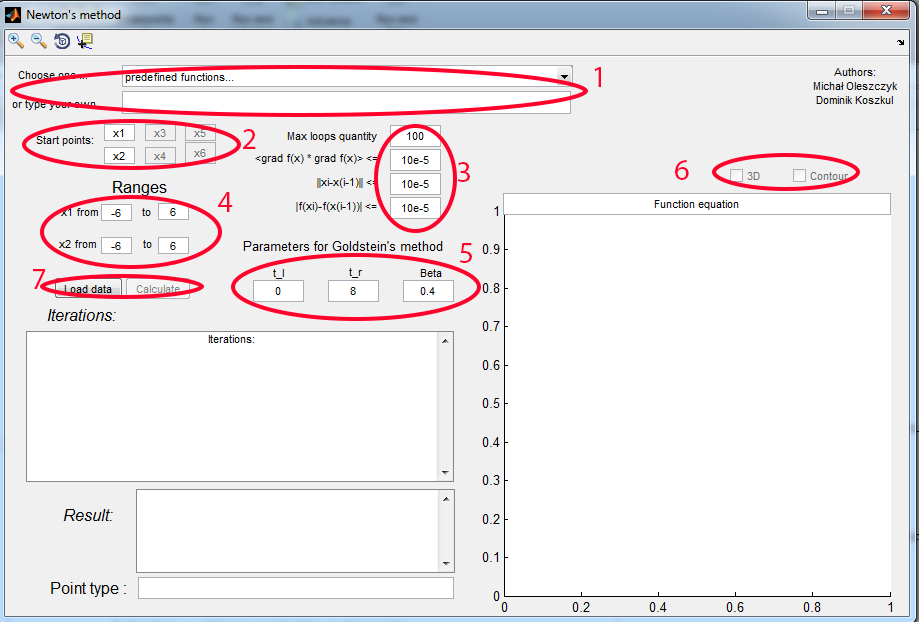
\includegraphics[scale=0.3]{images/program.png}
\caption{GUI of our program}
\label{program}
\end{center}		
\end{figure}
To start computing the user should go through a few steps:
\begin{enumerate}
\item choose one of predefined functions or type own (number 1 in figure \ref{program}),
\item click 'load data' button (number 7 in figure \ref{program}),
\item set starting points (number 2 in figure \ref{program}),
\item set accuracy for each stop criteria or leave default (number 3 in figure \ref{program}),
\item set ranges if $n < 3$ (number 4 in figure \ref{program}),
\item set parameters for method, which counts optimal step length in every iteration (number 5 in figure \ref{program}),
\item set plot type if $n < 3$ (number 6 in figure \ref{program}),
\item start calculations by push 'Calculate' button (number 7 in figure \ref{program}).
\end{enumerate}
\textbf{Select $\varepsilon$ (number 3 in figure \ref{program})} \\
The smaller $\varepsilon$ the better results but longer calculations. This constraint should be bigger than Matlab computing accuracy. Default is set $10^{-5}$ which is sufficient value and gives good results. \\

\textbf{Select ranges (number 4 in figure \ref{program})} \\
If user types or choose function which has $n < 3$ he can plot this functions and see steps generated during finding minimum. Ranges depends on chosen function. $x_1,x_2 \in [-6,6]$ are default values. \\

\textbf{Select Goldstein's method parameters (number 5 in figure \ref{program})}\\
Default values are $\tau_l=0$, $\tau_r=8$ and $\beta=0.4$ and provided correct calculations for most of chosen points. Rules to choose ranges are described in subsection \ref{MC}. The bigger $\beta$ the better results and longer calculations. With bigger $\beta$ algorithm may not find optimal point because method to find optimal step length will give very small steps and algorithm will not manage to reach minimum point.

\section{Examples}
\subsection{Function with four local minima}
Function equation:
\begin{equation}
y=x_1^4+x_2^4-0.62x_1^2-0.62x_2^2
\end{equation}

Function figures:
	\begin{figure}[H]
		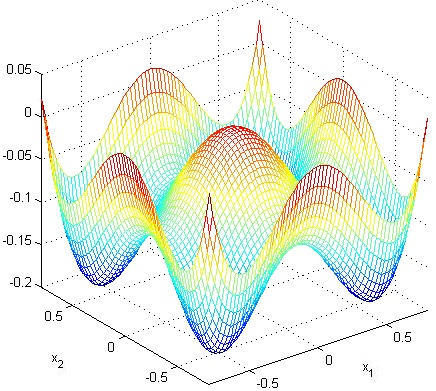
\includegraphics[width=12cm]{four_3d.jpg}
		\caption{Analyzed function 3D view.}
	\end{figure}
	\begin{figure}[H]
			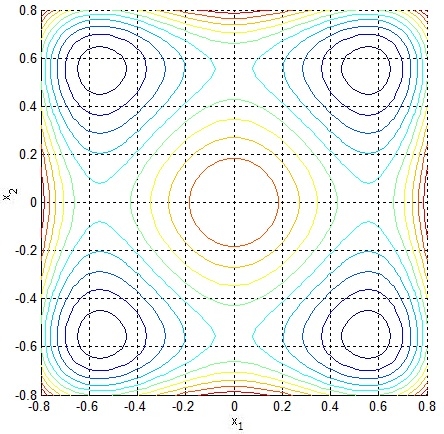
\includegraphics[width=12cm]{four_cont.jpg}
		\caption{Analyzed function contour view.}
	\end{figure}	

	\begin{table}[H]
		Results: \\ \\
		\begin{tabularx}{\textwidth}{c|X|c|c|c|c|}
			iteration & point coordinates & function value & $C_1$ value & $C_2$ value & $C_3$ value\\
			\hline
			0 & $1, 1$ & $0.76$ & $0.132$ & - & - \\
			\hline					
			1 & $0.743, 0.743$ & $-0.074$ & $0.132$ & $0.363$ & $0.834$ \\ 
			\hline 
			2 & $0.61, 0.61$ & $-0.185$ & $0.0358$ & $0.189$ & $0.11$ \\ 
			\hline
			3 & $5.63\cdot10^{-1}, 5.63\cdot10^{-1}$  & $-1.92\cdot10^{-1}$ & $4.36\cdot10^{-3}$ & $6.6\cdot10^{-2}$ & $7.5\cdot10^{-3}$ \\ 
			\hline
			4 & $5.63\cdot10^{-1}, 5.63\cdot10^{-1}$  & $-1.92\cdot10^{-1}$ &
			$7.35\cdot10^{-5}$ & $6.6\cdot10^{-2}$ & $7.5\cdot10^{-3}$ \\ \hline
		\end{tabularx}	
	\end{table}		
	\begin{table}[H]
		\begin{tabularx}{\textwidth}{c|X|c|c|c|c|}
			iteration & point coordinates & function value & $C_1$ value & $C_2$ value & $C_3$ value\\
			\hline	
			0 & $-1, 1$ & $0.76$ & $0.132$ & - & - \\
			\hline					
			1 & $-0.743, 0.743$ & $-0.074$ & $0.132$ & $0.363$ & $0.834$ \\ 
			\hline 
			2 & $-0.61, 0.61$ & $-0.185$ & $0.0358$ & $0.189$ & $0.11$ \\ 
			\hline
			3 & $-5.63\cdot10^{-1}, 5.63\cdot10^{-1}$  & $-1.92\cdot10^{-1}$ & $4.36\cdot10^{-3}$ & $6.6\cdot10^{-2}$ & $7.5\cdot10^{-3}$ \\ 
			\hline
			4 & $-5.63\cdot10^{-1}, 5.63\cdot10^{-1}$  & $-1.92\cdot10^{-1}$ &
			$7.35\cdot10^{-5}$ & $6.6\cdot10^{-2}$ & $7.5\cdot10^{-3}$ \\ \hline
		\end{tabularx}		 
	\end{table}
	\begin{table}[H]
		\begin{tabularx}{\textwidth}{c|X|c|c|c|c|}
			iteration & point coordinates & function value & $C_1$ value & $C_2$ value & $C_3$ value\\
			\hline	
			0 & $-1, -1$ & $0.76$ & $0.132$ & - & - \\
			\hline					
			1 & $-0.743, -0.743$ & $-0.074$ & $0.132$ & $0.363$ & $0.834$ \\ 
			\hline 
			2 & $-0.61, -0.61$ & $-0.185$ & $0.0358$ & $0.189$ & $0.11$ \\ 
			\hline
			3 & $-5.63\cdot10^{-1}, -5.63\cdot10^{-1}$  & $-1.92\cdot10^{-1}$ & $4.36\cdot10^{-3}$ & $6.6\cdot10^{-2}$ & $7.5\cdot10^{-3}$ \\ 
			\hline
			4 & $-5.63\cdot10^{-1}, -5.63\cdot10^{-1}$  & $-1.92\cdot10^{-1}$ &
			$7.35\cdot10^{-5}$ & $6.6\cdot10^{-2}$ & $7.5\cdot10^{-3}$ \\ \hline
		\end{tabularx}		 
	\end{table}
	\begin{table}[H]
		\begin{tabularx}{\textwidth}{c|X|c|c|c|c|}
			iteration & point coordinates & function value & $C_1$ value & $C_2$ value & $C_3$ value\\
			\hline	
			0 & $1, -1$ & $0.76$ & $0.132$ & - & - \\
			\hline					
			1 & $0.743, -0.743$ & $-0.074$ & $0.132$ & $0.363$ & $0.834$ \\ 
			\hline 
			2 & $0.61, -0.61$ & $-0.185$ & $0.0358$ & $0.189$ & $0.11$ \\ 
			\hline
			3 & $5.63\cdot10^{-1}, -5.63\cdot10^{-1}$  & $-1.92\cdot10^{-1}$ & $4.36\cdot10^{-3}$ & $6.6\cdot10^{-2}$ & $7.5\cdot10^{-3}$ \\ 
			\hline
			4 & $5.63\cdot10^{-1}, -5.63\cdot10^{-1}$  & $-1.92\cdot10^{-1}$ &
			$7.35\cdot10^{-5}$ & $6.6\cdot10^{-2}$ & $7.5\cdot10^{-3}$ \\ \hline
		\end{tabularx}		 
	\end{table}
	When we chose starting point at $x_1=0, x_2=0$ then program returned: 'local maximum. Computation stopped'. This is caused by checking Silvester's criterion. Even if algorithm find local extrema it can distinguish maxima or minima. 
	
	\begin{figure}[H]
		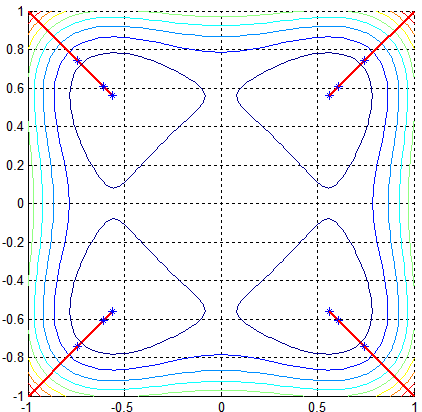
\includegraphics[width=13.5cm]{four_results.png}
		\caption{Location of four minima.}
	\end{figure}


\subsection{Himmelblau modification function}
Function equation:
\begin{equation}
	y=(x_1^2+x_2-11)^2 +(x_1+x_2^2-7)^2
\end{equation}

Function figures:
\begin{figure}[H]
	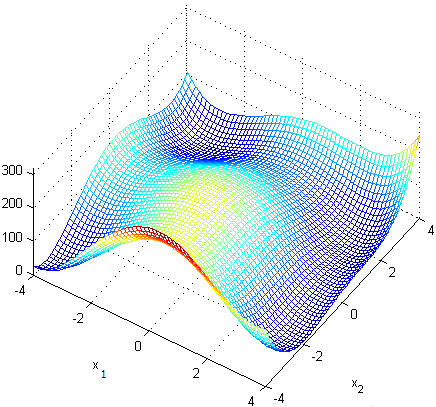
\includegraphics[width=8cm]{himm.png}
	\caption{Analyzed function 3D view.}
\end{figure}
\begin{figure}[H]
	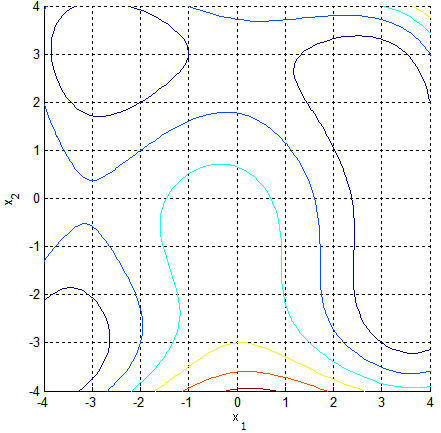
\includegraphics[width=8cm]{himm_count.png}
	\caption{Analyzed function contour view.}
\end{figure}

\begin{table}[H]
	Results: \\ \\
	\begin{tabularx}{\textwidth}{c|X|c|c|c|c|}
		iteration & point coordinates & function value & $C_1$ value & $C_2$ value & $C_3$ value\\
		\hline
		0 & $4, 4$ & $250$ & $1.867$ & - & - \\
		\hline					
		1 & $3.1, 2.901$ & $25.451$ & $1.867$ & $1.367$ & $224.55$ \\
		\hline
		2 & $2.957, 2.309$  & $1.666$ & $0.403$ & $0.635$ & $23.785$ \\ 
		\hline
		3 & $2.987 ,2.055$ & $4.53\cdot10^{-2}$ & $6.52\cdot10^{-2}$ & $2.55\cdot10^{-1}$  & $1.62$ \\
		\hline
		4 & $3, 2$ & $7.29\cdot10^{-5}$ & $3\cdot10^{-3}$ & $5.47\cdot10^{-2}$ & $4.53\cdot10^{-2}$ \\
		\hline
		5 & $3, 2$ & $7.29\cdot10^{-5}$ & $5.28\cdot10^{-6}$ & $5.47\cdot10^{-2}$ & $4.53\cdot10^{-2}$\\
		\hline
	\end{tabularx}	
\end{table}		

\begin{table}[H]
	\begin{tabularx}{\textwidth}{c|X|c|c|c|c|}
		iteration & point coordinates & function value & $C_1$ value & $C_2$ value & $C_3$ value\\
		\hline
		0 & $4, -4$ & $170$ & $1.379$ & - & - \\
		\hline
		1 & $3.687, -2.868$ & $24.212$ & $1.379$ & $1.174$ & $145.788$ \\ 
		\hline
		2 & $3.615, -2.215$ & $2.331$ & $0.432$ & $0.657$ & $21.881$ \\
		\hline
		3 & $3.591, -1.921$ & $7.99\cdot10^{-2}$ & $8.68\cdot10^{-2}$ & $0.295$ & $2.251$ \\
		\hline
		4 & $3.585, -1.852$ & $2.13\cdot10^{-4}$ & $4.81\cdot10^{-3}$ & $6.94\cdot10^{-2}$ & $7.97\cdot10^{-2}$ \\
		\hline
		5 & $3.585, -1.852$ & $2.13\cdot10^{-4}$ & $1.47\cdot10^{-5}$ & $6.94\cdot10^{-2}$ & $7.97\cdot10^{-2}$ \\ 
		\hline
	\end{tabularx}	
\end{table}	

\begin{table}[H]
	\begin{tabularx}{\textwidth}{c|X|c|c|c|c|}
		iteration & point coordinates & function value & $C_1$ value & $C_2$ value & $C_3$ value\\
		\hline
		0 & $-4, -4$ & $26$ & $3.43$ & - & - \\
		\hline
		1 & $-3.822, -3.442$ & $1.079$ & $0.343$ & $0.586$ & $24.921$ \\
		\hline
		2 & $-3.782, -3.294$ & $4.61\cdot10^{-3}$ & $2.36\cdot10^{-2}$ & $0.154$ & $1.074$ \\
		\hline
		3 & $-3.779, -3.283$ & $1.13\cdot10^{-7}$ & $1.19\cdot10^{-4}$ & $1.09\cdot10^{-2}$ & $4.61\cdot10^{-3}$ \\ 
		\hline
		4 & $-3.779, -3.283$ & $1.13\cdot10^{-7}$ & $2.93\cdot10^{-9}$ & $1.09\cdot10^{-2}$ & $4.61\cdot10^{-3}$ \\
		\hline
	\end{tabularx}	
\end{table}	

\begin{table}[H]
	\begin{tabularx}{\textwidth}{c|X|c|c|c|c|}
		iteration & point coordinates & function value & $C_1$ value & $C_2$ value & $C_3$ value\\
		\hline
		0 & $-4, 4$ & $106$ & $1.078$ & - & - \\
		\hline
		1 & $-3.193, 3.347$ & $7.469$ & $1.078$ & $1.038$ & $98.531$ \\
		\hline
		2 & $-2.867, 3.15$ & $0.139$ & $0.145$ & $0.381$ & $7.329$ \\
		\hline
		3 & $-2.807, 3.132$ & $1.23\cdot10^{-4}$ & $3.92\cdot10^{-3}$ & $6.26\cdot10^{-2}$ & $0.139$ \\
		\hline
		4 & $-2.807, 3.132$ & $1.23\cdot10^{-4}$ & $3.8\cdot10^{-6}$ & $6.26\cdot10^{-2}$ & $0.139$ \\ 
		\hline
	\end{tabularx}	
\end{table}	
When we chose starting point at $x_1=-3, x_2=0$ or $x_1=0.1, x_2=2.8$ then program returned: 'local minimum or maximum does not exist'. This is caused by saddle points there. Situation can be seen on figure 6. And at point $x_1=0, x_2=0$ we found local maxima. Program returned: 'local maximum. Computation stopped'. 
\begin{figure}[H]
	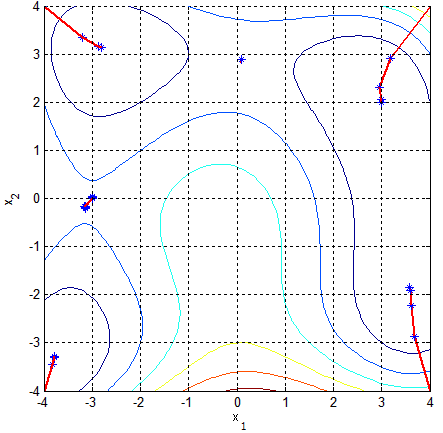
\includegraphics[width=16cm]{himm_results.png}
		\caption{Location of four minima and saddle point.}
\end{figure} 

\subsection{Geem test function}
Function equation:
\begin{equation}
y=4x_1^2-2.1x_1^4+\frac{1}{3}x_1^6+x_1x_2-4x_2^2+4x_2^4
\end{equation}

Function figures:
\begin{figure}[H]
	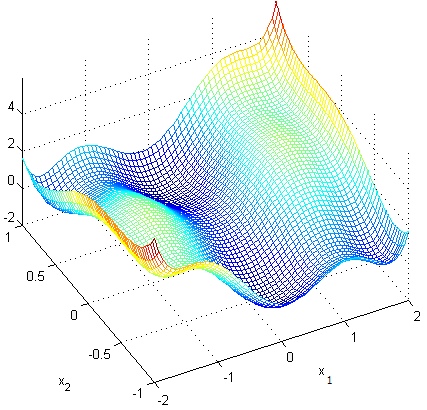
\includegraphics[width=8cm]{gem_3D.png}
	\caption{Analyzed function 3D view.}
\end{figure}
\begin{figure}[H]
	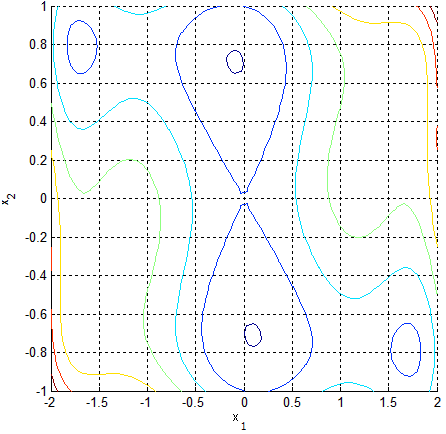
\includegraphics[width=8cm]{gem_cont.png}
	\caption{Analyzed function contour view.}
\end{figure}


	\begin{table}[H]
		Results: \\\\
		\begin{tabularx}{\textwidth}{c|X|c|c|c|c|}
			iteration & point coordinates & function value & $C_1$ value & $C_2$ value & $C_3$ value\\
			\hline
			0 & $0.5, 0.9$ & $0.708$ & $2.69$ & - & - \\
			\hline
			1 & $-0.318, 0.846$ & $-0.699$ & $2.69$ & $0.82$ & $1.407$ \\
			\hline
			2 & $-7.47\cdot10^{-2}, 0.75$ & $-1.017$ & $8.942\cdot10^{-2}$ & $0.262$ & $0.319$ \\
			\hline
			3 & $-8.82\cdot10^{-2}, 0.72$ & $-1.031$ & $1.47\cdot10^{-3}$ & $3.36\cdot10^{-2}$ & $1.33\cdot10^{-2}$ 	\\
			\hline		
			4 & $-8.82\cdot10^{-2}, 0.72$ & $-1.031$ & $5.11\cdot10^{-5}$ & $3.36\cdot10^{-2}$ & $1.33\cdot10^{-2}$ 	\\
			\hline		
		\end{tabularx}	
	\end{table}	

	\begin{table}[H]
		\begin{tabularx}{\textwidth}{c|X|c|c|c|c|}
			iteration & point coordinates & function value & $C_1$ value & $C_2$ value & $C_3$ value\\
			\hline
			0 & $-0.5, -0.9$ & $0.708$ & $2.69$ & - & - \\
			\hline
			1 & $0.318, -0.846$ & $-0.699$ & $2.69$ & $0.82$ & $1.407$ \\
			\hline
			2 & $7.47\cdot10^{-2}, -0.75$ & $-1.017$ & $8.942\cdot10^{-2}$ & $0.262$ & $0.319$ \\
			\hline
			3 & $8.82\cdot10^{-2}, -0.72$ & $-1.031$ & $1.47\cdot10^{-3}$ & $3.36\cdot10^{-2}$ & $1.33\cdot10^{-2}$ 	\\
			\hline		
			4 & $8.82\cdot10^{-2}, -0.72$ & $-1.031$ & $5.11\cdot10^{-5}$ & $3.36\cdot10^{-2}$ & $1.33\cdot10^{-2}$ 	\\
			\hline		
		\end{tabularx}	
	\end{table}
	
	\begin{table}[H]
		\begin{tabularx}{\textwidth}{c|X|c|c|c|c|}
			iteration & point coordinates & function value & $C_1$ value & $C_2$ value & $C_3$ value\\
			\hline
			0 & $-2, 1$ & $1.733$ & $5.55\cdot10^{-2}$ & - & - \\
			\hline
			1 & $-1.822, 0.846$ & $-2.47\cdot10^{-2}$ & $5.55\cdot10^{-2}$ & $0.236$ & $1.758$ \\
			\hline
			2 & $-1.732, 0.8$ & $-0.207$ & $1.02\cdot10^{-2}$ & $0.101$ & $0.183$ \\ 
			\hline
			3 & $-1.705, 0.796$ & $-0.215$ & $6.92\cdot10^{-4}$ & $2.63\cdot10^{-2}$ & $7.95\cdot10^{-3}$ \\
			\hline
			4 & $-1.705, 0.796$ & $-0.215$ & $4.21\cdot10^{-6}$ & $2.63\cdot10^{-2}$ & $7.95\cdot10^{-3}$ \\
			\hline
		\end{tabularx}	
	\end{table}	

	\begin{table}[H]
		\begin{tabularx}{\textwidth}{c|X|c|c|c|c|}
			iteration & point coordinates & function value & $C_1$ value & $C_2$ value & $C_3$ value\\
			\hline
			0 & $2, -1$ & $1.733$ & $5.55\cdot10^{-2}$ & - & - \\
			\hline
			1 & $1.822, -0.846$ & $-2.47\cdot10^{-2}$ & $5.55\cdot10^{-2}$ & $0.236$ & $1.758$ \\
			\hline
			2 & $1.732, -0.8$ & $-0.207$ & $1.02\cdot10^{-2}$ & $0.101$ & $0.183$ \\ 
			\hline
			3 & $1.705, -0.796$ & $-0.215$ & $6.92\cdot10^{-4}$ & $2.63\cdot10^{-2}$ & $7.95\cdot10^{-3}$ \\
			\hline
			4 & $1.705, -0.796$ & $-0.215$ & $4.21\cdot10^{-6}$ & $2.63\cdot10^{-2}$ & $7.95\cdot10^{-3}$ \\
			\hline
		\end{tabularx}	
	\end{table}	

	\begin{table}[H]
		\begin{tabularx}{\textwidth}{c|X|c|c|c|c|}
			iteration & point coordinates & function value & $C_1$ value & $C_2$ value & $C_3$ value\\
			\hline
			0 & $2, 1$ & $5.733$ & $0.101$ & - & - \\
			\hline
			1 & $1.798, 0.755$ & $2.624$ & $0.101$ & $0.317$ & $3.109$ \\
			\hline
			2 & $1.677, 0.625$ & $2.15$ & $3.17\cdot10^{-2}$ & $0.178$ & $0.474$ \\
			\hline
			3 & $1.621, 0.576$ & $2.106$ & $5.48\cdot10^{-3}$ & $7.4\cdot10^{-2}$ & $4.46\cdot10^{-2}$ \\
			\hline
			4 & $1.608, 0.567$ & $2.104$ & $2.3\cdot10^{-4}$ & $1.52\cdot10^{-2}$ & $1.31\cdot10^{-3}$ \\
			\hline
			5 & $1.608, 0.567$ & $2.104$ & $6.52\cdot10^{-7}$ & $1.52\cdot10^{-2}$ & $1.31\cdot10^{-3}$ \\
			\hline
						
 		\end{tabularx}	
	\end{table}

	\begin{table}[H]
		\begin{tabularx}{\textwidth}{c|X|c|c|c|c|}
			iteration & point coordinates & function value & $C_1$ value & $C_2$ value & $C_3$ value\\
			\hline
			0 & $-2, -1$ & $5.733$ & $0.101$ & - & - \\
			\hline
			1 & $-1.798, -0.755$ & $2.624$ & $0.101$ & $0.317$ & $3.109$ \\
			\hline
			2 & $-1.677, -0.625$ & $2.15$ & $3.17\cdot10^{-2}$ & $0.178$ & $0.474$ \\
			\hline
			3 & $-1.621, -0.576$ & $2.106$ & $5.48\cdot10^{-3}$ & $7.4\cdot10^{-2}$ & $4.46\cdot10^{-2}$ \\
			\hline
			4 & $-1.608, -0.567$ & $2.104$ & $2.3\cdot10^{-4}$ & $1.52\cdot10^{-2}$ & $1.31\cdot10^{-3}$ \\
			\hline
			5 & $-1.608, -0.567$ & $2.104$ & $6.52\cdot10^{-7}$ & $1.52\cdot10^{-2}$ & $1.31\cdot10^{-3}$ \\
			\hline		
		\end{tabularx}	
	\end{table}
When we chose starting point at $x_1=-1, x_2=0.7$ or $x_1=1, x_2=-0.7$ or $x_1=0, x_2=0$ then program returned: 'local minimum or maximum does not exist'. This is caused by saddle points there. Situation can be seen on figure 9. On the other hand start points at $x_1=1.25, x_2=0.2$ and $x_1=-1.25, x_2=-0.2$ program described as neighbourhood of local maxima.
	
\begin{figure}[H]
	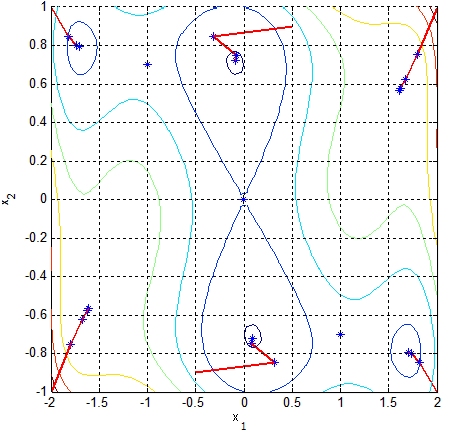
\includegraphics[width=16cm]{gem_results.png}
	\caption{Location of four minima and saddle points.}
\end{figure}		

\subsection{Practical example - spring-carts system}
Interpretation:

Figure 10 shows two frictionless rigid bodies (carts) A and B connected by three linear elastic springs having spring constants $k_1n k_2, k_3$. The springs are at their natural positions when the applied force $P$ is zero. The task is to find the displacement $x_1$ and $x_2$ under the force $P$ by using principle of minimum potential energy.

\begin{figure}[H]
	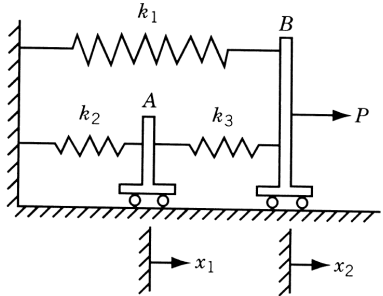
\includegraphics[width=16cm]{springs.png}
	\caption{Spring-cart system.}
\end{figure}

Function equation:
\begin{equation}
y=(\frac{1}{2}k_2x_1^2+\frac{1}{2}k_3(x_2-x_1)^2+\frac{1}{2}k_1x_2^2)-Px_2
\end{equation}
Lets assume:
$k_1=12, k_2=30, k_3=15, P=100$.
\\\\
Function figures:
\begin{figure}[H]
	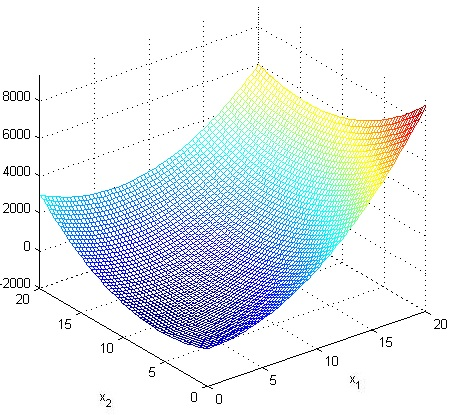
\includegraphics[width=8cm]{springs_3D.jpg}
	\caption{Analyzed function 3D view.}
\end{figure}
\begin{figure}[H]
	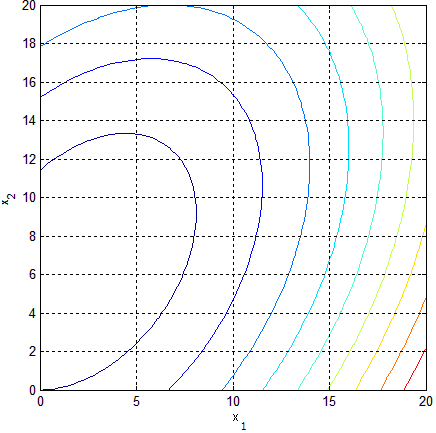
\includegraphics[width=8cm]{springs_cont.png}
	\caption{Analyzed function contour view.}
\end{figure}

	\begin{table}[H]
		\begin{tabularx}{\textwidth}{c|X|c|c|c|c|}
			iteration & point coordinates & function value & $C_1$ value & $C_2$ value & $C_3$ value\\
			\hline
			0 & $10, 10$ & $500$ & $101.736$ & - & - \\
			\hline
			1 & $2.083, 3.75$ & $-187.5$ & $101.736$ & $10.086$ & $787.5$ \\
			\hline
			2 & $2.083, 3.75$ & $-187.5$ & $5.6.52\cdot10^{-31}$ & $10.086$ & $787.5$ \\
			\hline		
		\end{tabularx}	
	\end{table}

\begin{figure}[H]
	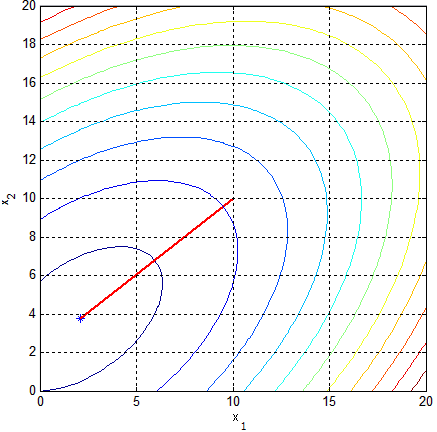
\includegraphics[width=16cm]{spirngs_results.png}
	\caption{Founded minimum.}
\end{figure}	

Example taken from "Engineering Optimization: Theory and Practice" (Authors: Singiresu S. Rao,S. S. Rao).

	
\begin{thebibliography}{99}
\bibitem{mathematics} http://math.stackexchange.com/questions/873467/goldstein-test-in-nonlinear-programming
\end{thebibliography}
	
	
\end{document}